\section{Avaliação dos Resultados}

Com as metodologias explicadas, é possível analisar o desempenho de cada uma das 
estratégias em partidas controladas de 21 dentro da aplicação que foi criada. Antes 
de ir direto para os resultado, seria interessante como os testes foram realizados 
e configurados para cada uma das situações.

\newpage

\subsection{Analisando a interface de testes}

\begin{figure}[ht] 
    \centering
    
\includegraphics[width=\linewidth]{main_screen.jpg}
    \caption{Tela do menu principal}
    \label{fig:main_menu}
\end{figure}

Na figura \ref{fig:main_menu} temos a tela do menu inicial do jogo. Aqui temos 
duas opções que são relevantes: \emph{New game} e \emph{Settings}

\begin{figure}[ht] 
    \centering
    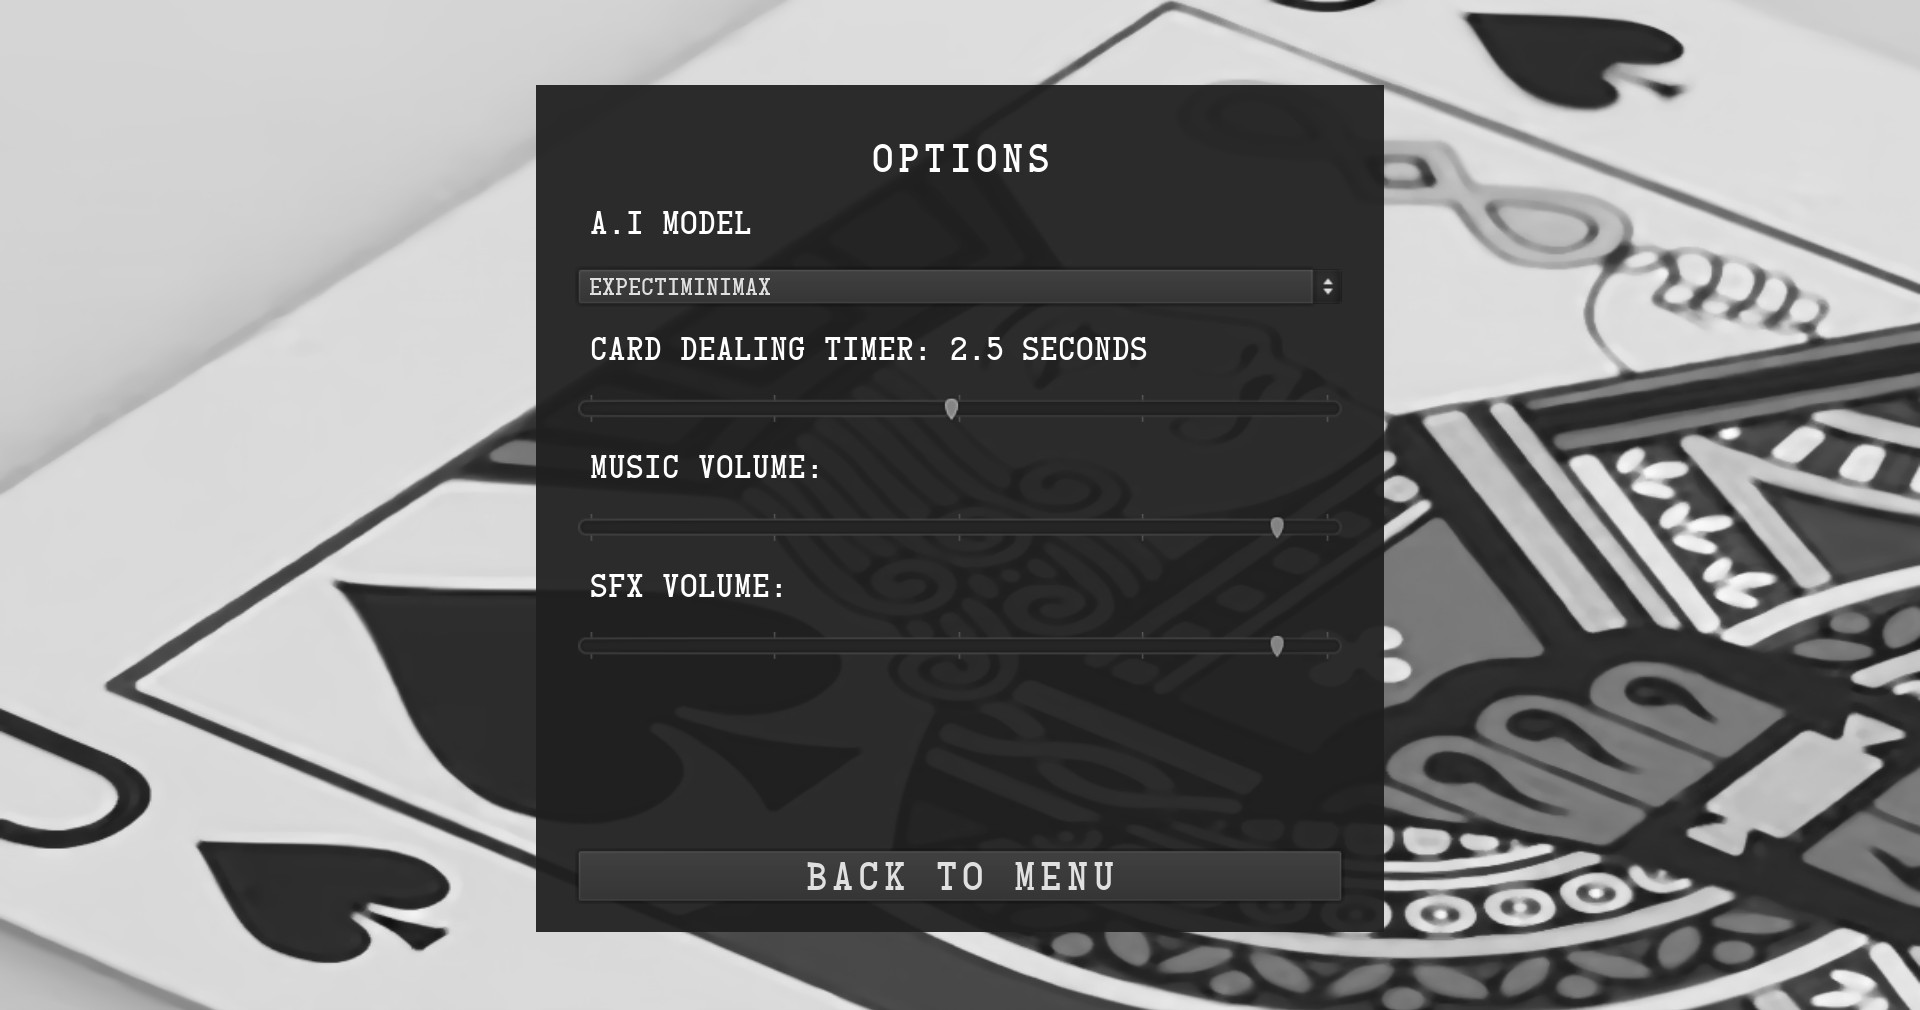
\includegraphics[width=\linewidth]{settings.jpg}
    \caption{Tela do menu de configurações}
    \label{fig:settings}
\end{figure}

Na tela de configurações é possível escolher qual será a estratégia 
empregada pelo inimigo, que no caso as opções são: \emph{Expectiminimax}, 
\emph{Genetic Learning} e \emph{Counting Cards}.

Além disso, é também configurar outras opções do jogo, como o tempo para 
as cartas descerem e o volume do jogo.

Por fim vamos a atração principal, o jogo em si:

\begin{figure}[ht] 
    \centering
    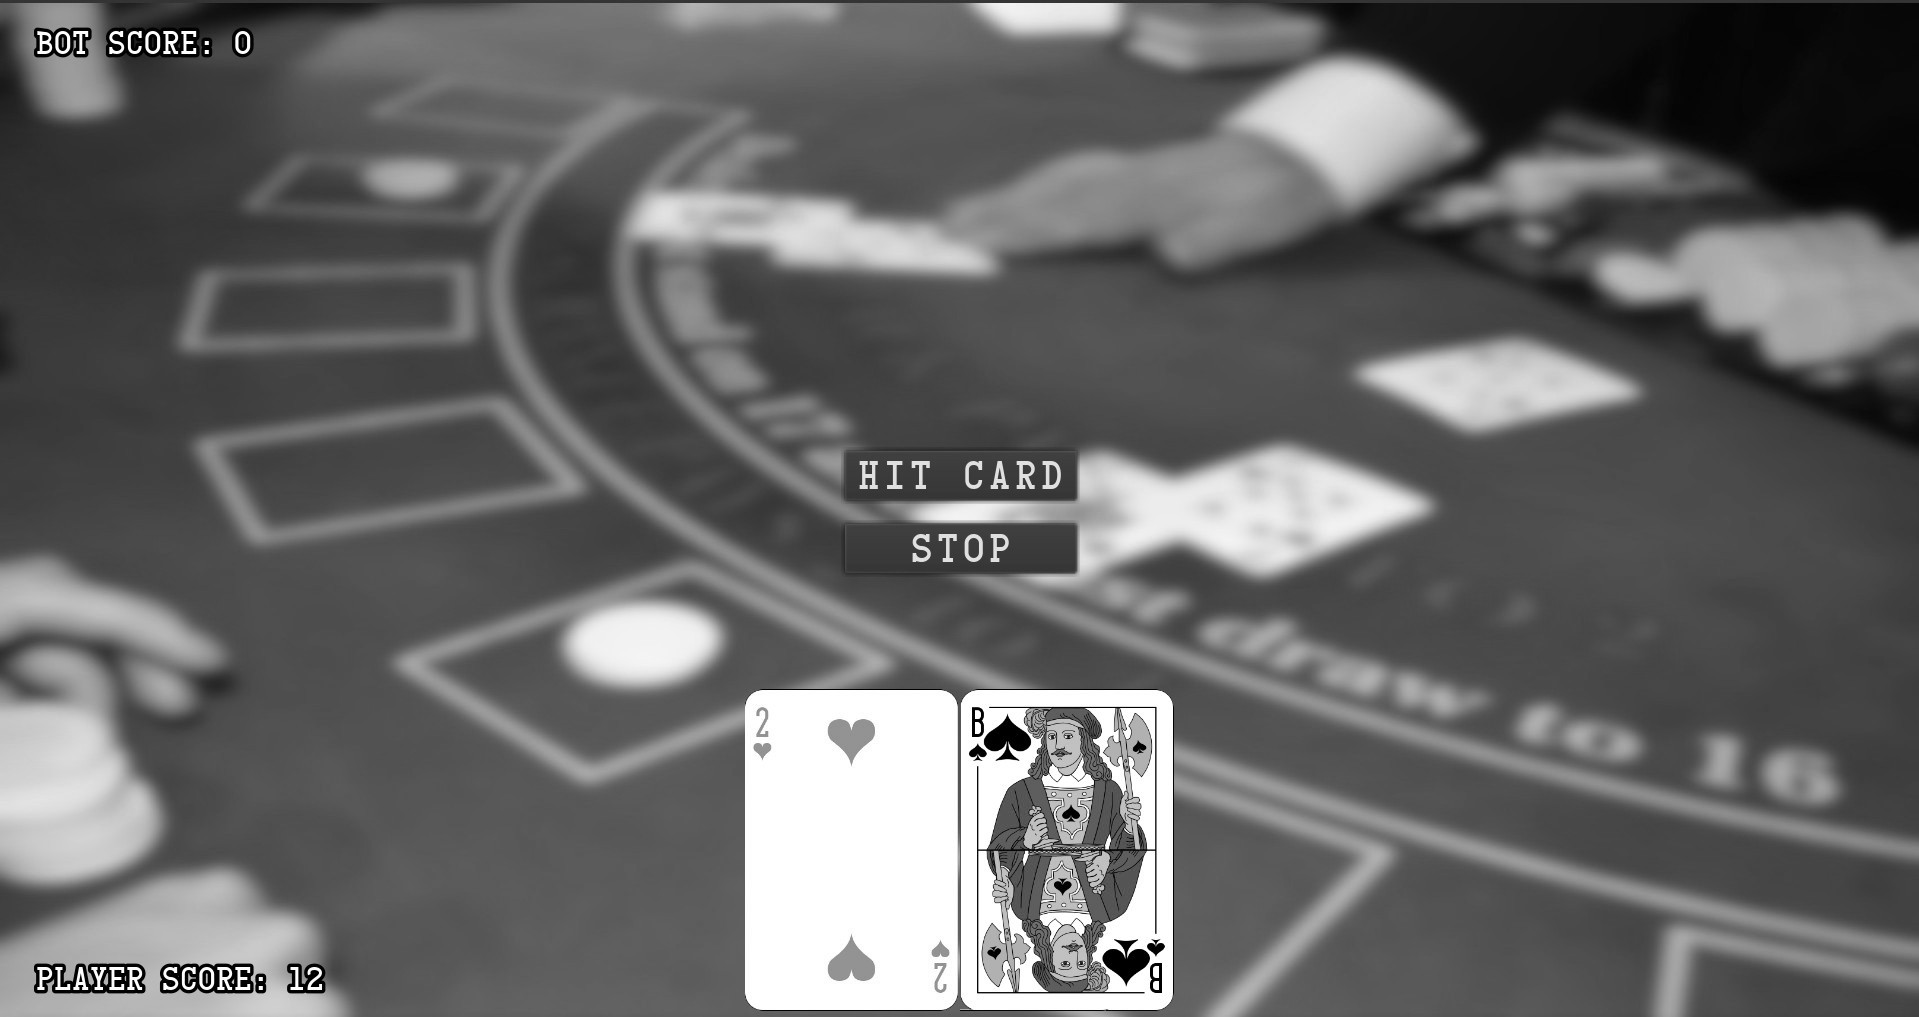
\includegraphics[width=\linewidth]{game.jpg}
    \caption{Tela principal do jogo}
    \label{fig:game}
\end{figure}

Como é possível ver na figura \ref{fig:game}, o jogador (na parte inferior)
da tela, recebe duas cartas, enquanto que o inimigo(Inteligência Artificial)
recebe duas cartas sendo uma delas viradas para cima e a outra para baixo. Em 
outras palavras o inimigo sempre será o dono da mesa(dealer).

Acima das carta, o jogador tem duas opções:
\begin{itemize}
    \item \emph{Hit}: O jogador receberá uma carta, se o jogador ficar com um 
    placar superior a 21 pontos, o jogo irá terminar e a tela de Fim de jogo (Game Over)
    irá aparecer na tela. Caso contrário o jogo irá somar o resultado das cartas ao placar 
    e exibir na tela 
    \item \emph{Stand}: O jogador irá passar seu turno para o oponente e não poderá 
    comprar mais cartas.
\end{itemize}

\begin{figure}[ht] 
    \centering
    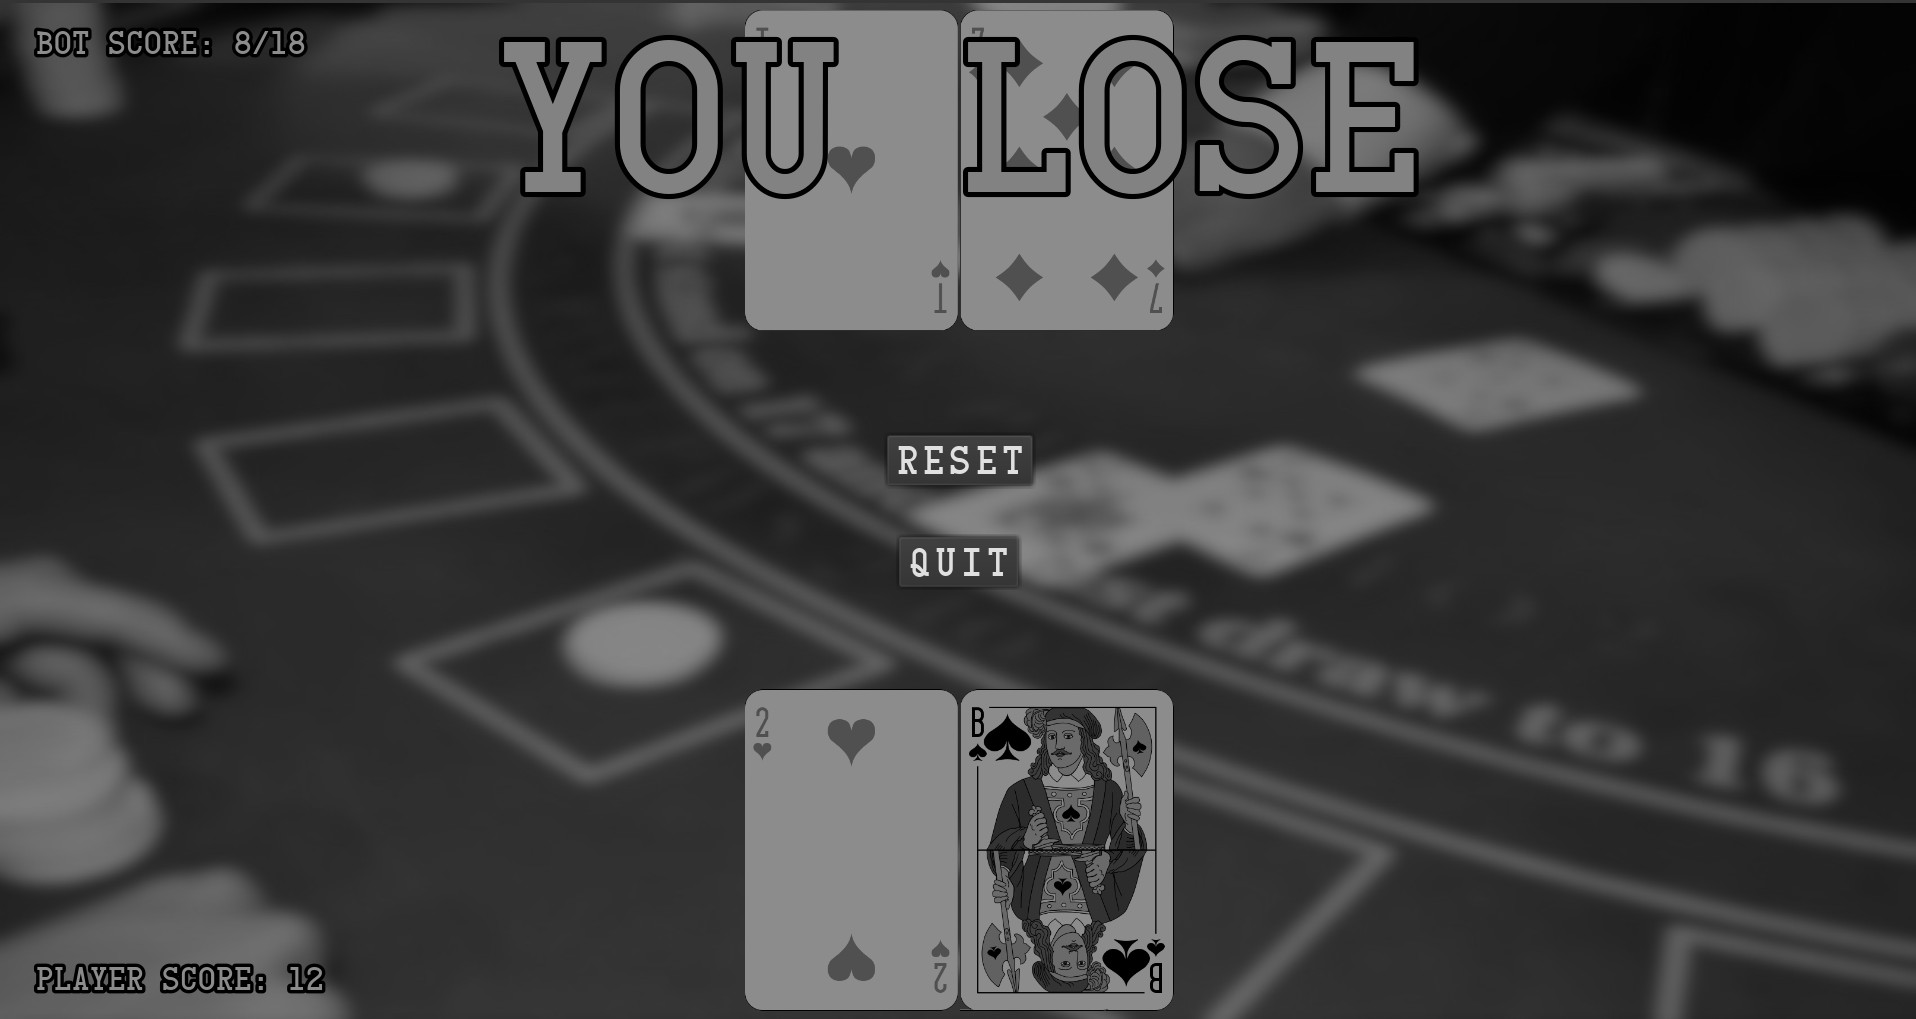
\includegraphics[width=\linewidth]{you_lose.jpg}
    \caption{Tela quando o jogador perde}
    \label{fig:you_lose}
\end{figure}

\begin{figure}[ht] 
    \centering
    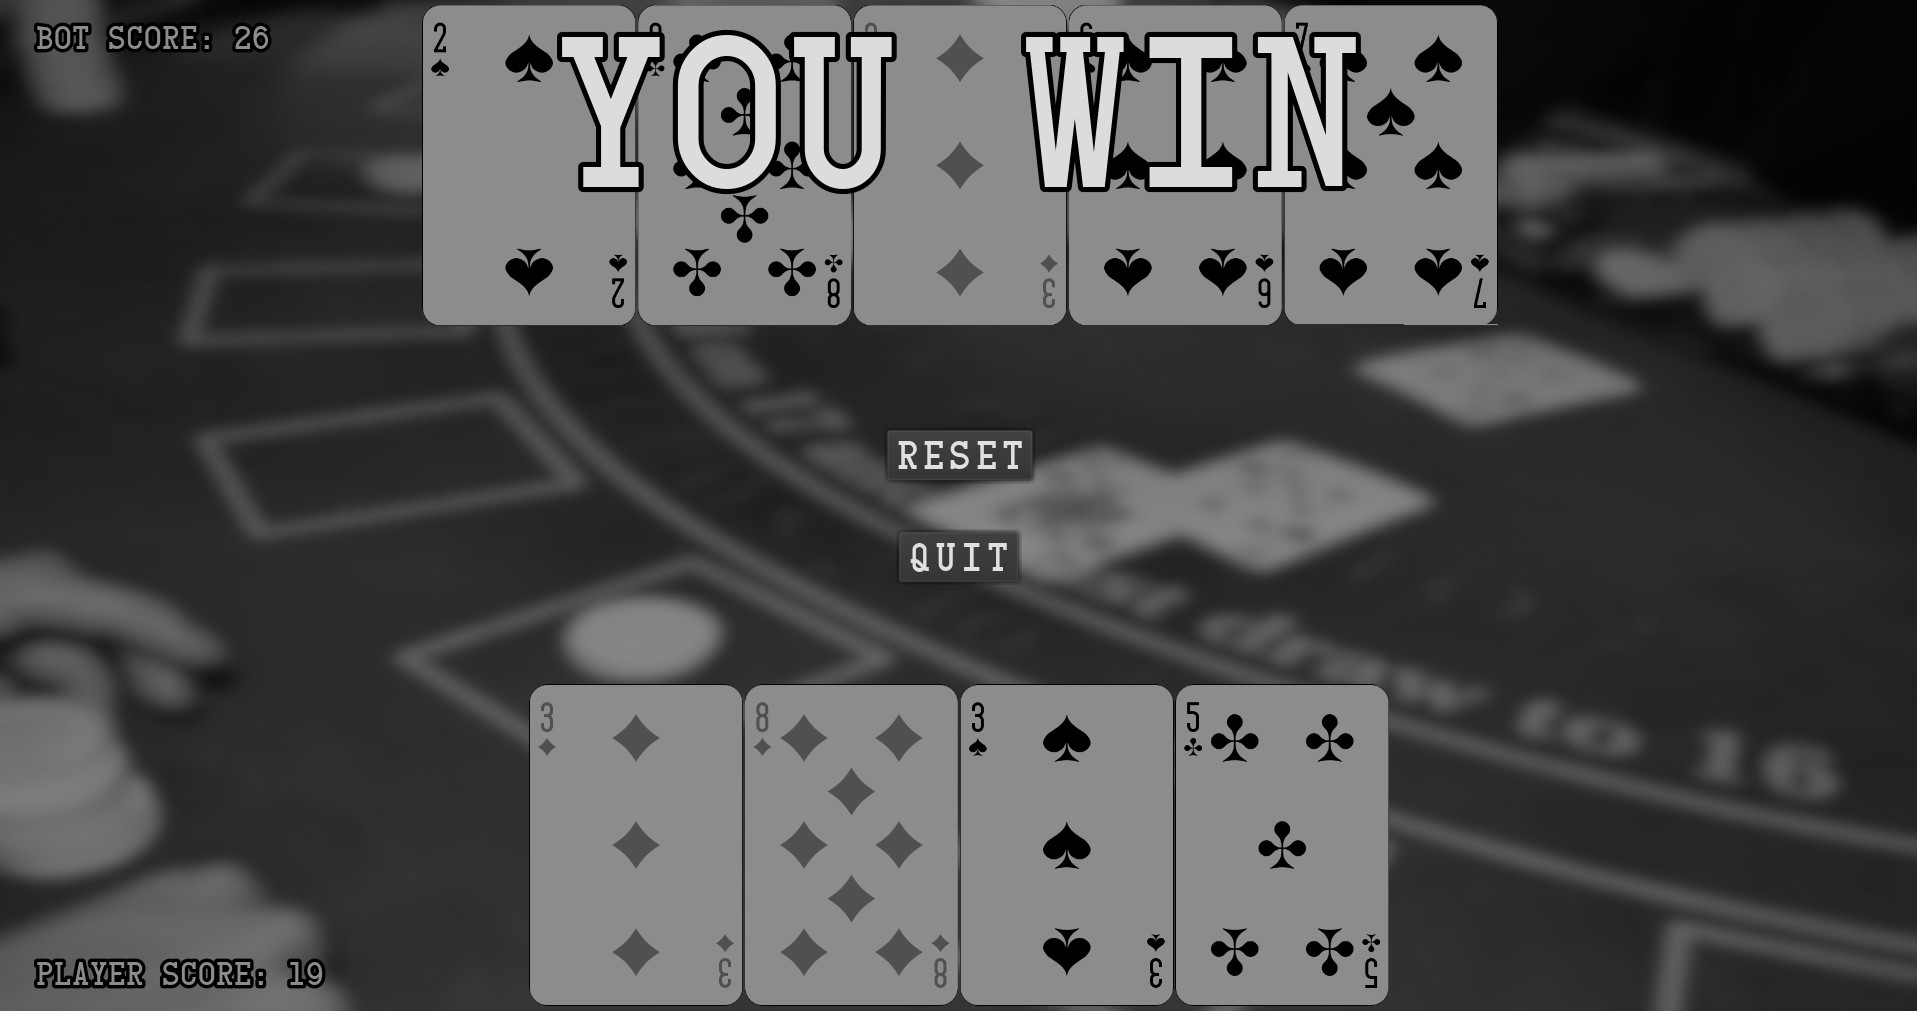
\includegraphics[width=\linewidth]{you_win.jpg}
    \caption{Tela quando o jogador ganha}
    \label{fig:you_win}
\end{figure}

\subsection{Testes}

Eis a maneira em como foi realizado os testes, um total de cem(100) testes 
foram feitos para cada uma das estratégias diferentes e analisado a
porcentagem de vitória de cada uma das políticas, a tabela mostra como foi 
o resultado desses testes.

\begin{table}[htbp]
    \centering
    \caption{Resultados dos testes}
    \begin{tabular}{|c | c | c | c|} 
        \hline
        Estratégias & \multicolumn{3}{|c|}{\textbf{Porcentagem de vitória por número de testes}} \\ 
        \cline{2-4} 
          & 50 & 100 & 150 \\ 
        \hline
        Contar cartas  & 41.0\% & 41.4\% & 41.9\% \\
        \hline
        Expectiminimax & 38.4\% & 38.6\% & 38.9\% \\
        \hline
    \end{tabular}
    \label{tab:results}
\end{table}

Podemos notar que os resultados  \ref{tab:results}

